\chapter{Kinetika Kompleks: Rantai, Enzim, dan Osilasi}\label{ch:b3:complex-kinetics}

Segelas larutan yang diaduk berubah menjadi tak berwarna, lalu kuning
kecokelatan, lalu biru, lalu tak berwarna lagi, dan terus berbuat demikian
selama bermenit-menit; jika dituang ke sebuah cawan, campuran yang sama
menggambar spiral-spiral yang berputar dan merambat. Ketika Boris Belousov
menggambarkan reaksi semacam itu pada tahun 1951, naskahnya ditolak: menurut
penelaahnya, sebuah sistem kimia tidak mungkin bergerak bolak-balik, karena
sistem itu harus menurun ke arah kesetimbangan. Sistem itu memang menurun;
hanya saja tidak secara lurus. Bab ini membahas mekanisme bertahap banyak
yang zat-zat antaranya terbentuk kembali: \omterm{def:b3:complex-kinetics:chain}{reaksi berantai} dan ledakan,
molekul yang memerlukan tumbukan untuk terurai sendiri, \omterm{def:b3:complex-kinetics:enzyme}{enzim}, dan
\omterm{def:b3:complex-kinetics:oscillating}{reaksi-reaksi berosilasi}, beserta metode-metode untuk mengikuti reaksi yang
terlalu cepat untuk dicampur dengan tangan.

\begin{recall}
Jilid Tahun 1 mendefinisikan mekanisme reaksi sebagai urutan tahap elementer,
tahap penentu laju, pendekatan prakesetimbangan dan pendekatan keadaan
tunak, serta katalis. Jilid Tahun 2 menamai tahap-tahap rantai radikal
(inisiasi, propagasi, terminasi), inisiator radikal, dan panjang rantai
kinetik sebuah polimerisasi, serta mencocokkan garis kuadrat terkecil.
\Cref{ch:b3:rate-theories} memberikan \omterm{def:b3:rate-theories:tst}{teori keadaan transisi} dan batas difusi
sekitar \qty{e10}{L.mol^{-1}.s^{-1}}.
\end{recall}

\section{Reaksi berantai}

\begin{definition}[Reaksi berantai, pembawa rantai]\label{def:b3:complex-kinetics:chain}
Yang disebut \emph{reaksi berantai}\index{reaksi berantai} adalah reaksi yang
zat-zat antara reaktifnya, yaitu \emph{pembawa rantai}\index{pembawa rantai},
dibentuk kembali oleh sebuah siklus tahap propagasi, sehingga satu peristiwa
inisiasi mengubah banyak molekul pereaksi.
\end{definition}

Bodenstein mengukur pada tahun 1906 laju $\ce{H2 + Br2 -> 2 HBr}$ dan menemukan
sebuah hukum yang tidak mungkin dihasilkan oleh satu tahap saja: lajunya
tumbuh sebanding dengan $[\ce{Br2}]^{1/2}$ dan turun ketika HBr menumpuk.
Mekanismenya dituliskan pada tahun 1919:
\begin{center}
\begin{tabular}{lll}
inisiasi & $\ce{Br2 -> 2 Br}$ & $k_1$ \\
propagasi & $\ce{Br + H2 -> HBr + H}$ & $k_2$ \\
propagasi & $\ce{H + Br2 -> HBr + Br}$ & $k_3$ \\
inhibisi & $\ce{H + HBr -> H2 + Br}$ & $k_4$ \\
terminasi & $\ce{2 Br -> Br2}$ & $k_{-1}$
\end{tabular}
\end{center}
(tumbukan dengan benda ketiga M yang membawa energi masuk ke dan keluar dari
tahap inisiasi dan terminasi tidak dituliskan).

\begin{theorem}[Hukum laju hidrogen--bromin]\label{thm:b3:complex-kinetics:hbr}
Dengan pendekatan keadaan tunak untuk Br dan H, laju
$v = \frac12\,\dd[\ce{HBr}]/\dd t$ mekanisme itu adalah
\[
  v = \frac{k[\ce{H2}][\ce{Br2}]^{1/2}}{1 + k'[\ce{HBr}]/[\ce{Br2}]},
  \qquad k = k_2\Bigl(\frac{k_1}{k_{-1}}\Bigr)^{1/2},\ k' = \frac{k_4}{k_3}.
\]
\end{theorem}

\begin{proof}
Keadaan tunak untuk H: $k_2[\ce{Br}][\ce{H2}] = k_3[\ce{H}][\ce{Br2}] + k_4[\ce{H}][\ce{HBr}]$.
Keadaan tunak untuk Br:
$2k_1[\ce{Br2}] - k_2[\ce{Br}][\ce{H2}] + k_3[\ce{H}][\ce{Br2}] + k_4[\ce{H}][\ce{HBr}] - 2k_{-1}[\ce{Br}]^2 = 0$.
Jika kedua persamaan dijumlahkan, suku-suku propagasi saling meniadakan:
$k_1[\ce{Br2}] = k_{-1}[\ce{Br}]^2$, sehingga $[\ce{Br}] =
(k_1/k_{-1})^{1/2}[\ce{Br2}]^{1/2}$. Lalu $[\ce{H}] = k_2[\ce{Br}][\ce{H2}]/(k_3[\ce{Br2}] + k_4[\ce{HBr}])$ dan
\[
  \frac{\dd[\ce{HBr}]}{\dd t} = k_2[\ce{Br}][\ce{H2}] + k_3[\ce{H}][\ce{Br2}] - k_4[\ce{H}][\ce{HBr}] = 2k_3[\ce{H}][\ce{Br2}]
  = \frac{2k_2[\ce{Br}][\ce{H2}]}{1 + (k_4/k_3)[\ce{HBr}]/[\ce{Br2}]},
\]
dengan memakai persamaan pertama; menyubstitusikan $[\ce{Br}]$ memberikan hasilnya.
\end{proof}

\begin{omfigure}
\begin{tikzpicture}[font=\small, >=Stealth]
  \node[draw, circle, minimum size=9mm, omDef, thick] (br) at (0,0) {Br};
  \node[draw, circle, minimum size=9mm, omThm, thick] (h) at (4,0) {H};
  \draw[->, thick] (br) to[bend left=35] node[midway, above, align=center] {$+\,\ce{H2}$\\ $\to$ HBr} (h);
  \draw[->, thick] (h) to[bend left=35] node[midway, below, align=center] {$+\,\ce{Br2}$\\ $\to$ HBr} (br);
  \draw[->, thick, black!60] (-2.4,0) -- (br) node[pos=0, left, align=right] {inisiasi\\ $\ce{Br2 -> 2 Br}$};
  \draw[->, thick, black!60] (br) -- (0,-2.0) node[below, align=center] {terminasi\\ $\ce{2 Br -> Br2}$};
  \draw[->, thick, black!60, dashed] (h) -- (6.2,-1.2) node[below, align=center] {inhibisi\\ $\ce{H + HBr -> H2 + Br}$};
\end{tikzpicture}

{\small Siklus propagasi rantai hidrogen--bromin: setiap putaran memakai satu
\ce{H2} dan satu \ce{Br2}, menghasilkan dua HBr, dan mengembalikan atom bromin
yang memulainya. Inisiasi memasok pembawa ke dalam siklus, terminasi
menyingkirkannya; tahap inhibisi mengubah atom H kembali menjadi Br dengan
mengorbankan sebuah HBr yang sudah terbentuk.}
\end{omfigure}

\begin{omfigure}
\begin{tikzpicture}
\begin{axis}[name=ca, width=0.47\linewidth, height=5.2cm, xmin=0, xmax=800, ymin=0, ymax=1,
  axis lines=left, xlabel={$t$ (tereduksi)}, ylabel={$[\ce{HBr}]/2[\ce{H2}]_0$},
  tick label style={font=\small}, label style={font=\small}]
\addplot[omDef, thick] table[x=t, y expr=\thisrow{HBr}/2] {figdata/out/bachelor-3-chain-kinetics.dat};
\end{axis}
\begin{axis}[at={(ca.east)}, anchor=west, xshift=1.4cm, width=0.47\linewidth, height=5.2cm,
  xmin=0, xmax=60, ymin=0, ymax=2.2, axis lines=left, xlabel={$t$ (tereduksi)},
  ylabel={laju $\times 10^3$}, tick label style={font=\small}, label style={font=\small},
  legend style={font=\scriptsize, draw=none, at={(0.97,0.03)}, anchor=south east},
  legend cell align=left]
\addplot[omDef, thick] table[x=t, y expr=1000*\thisrow{v}] {figdata/out/bachelor-3-chain-kinetics.dat};
\addplot[omThm, thick, dashed] table[x=t, y expr=1000*\thisrow{vss}] {figdata/out/bachelor-3-chain-kinetics.dat};
\legend{mekanisme lengkap, hukum keadaan tunak}
\end{axis}
\end{tikzpicture}

{\small Mekanisme hidrogen--bromin yang diintegrasikan tahap demi tahap
(tetapan laju model, satuan tereduksi, $k' = 0.1$): konversi terhadap waktu
(kiri), dan laju $\frac12\dd[\ce{HBr}]/\dd t$ mekanisme lengkap dibandingkan dengan
hukum keadaan tunak (kanan). Setelah masa induksi, selama atom-atom bromin
menumpuk, keduanya berimpit dengan selisih kurang dari 1\,\%.}
\end{omfigure}

\begin{method}[Hukum laju mekanisme berantai]\label{met:b3:complex-kinetics:steady-state-chain}
\begin{enumerate}
  \item Tuliskan persamaan keadaan tunak untuk setiap \omterm{def:b3:complex-kinetics:chain}{pembawa rantai}.
  \item Jumlahkan persamaan-persamaan itu: tahap-tahap propagasi, yang hanya
        menukar satu pembawa dengan pembawa lain, saling meniadakan, sehingga
        tersisa inisiasi yang sama dengan terminasi; ini memberikan konsentrasi
        pembawa.
  \item Gunakan persamaan satu pembawa untuk menyatakan pembawa-pembawa lain.
  \item Tuliskan laju pembentukan sebuah produk dari tahap-tahap propagasi.
\end{enumerate}
\end{method}

Banyaknya siklus propagasi per peristiwa inisiasi, di sini $v/k_1[\ce{Br2}]$,
adalah panjang rantai kinetik dalam jilid Tahun 2; untuk reaksi
hidrogen--bromin nilainya berorde $10^3$ sampai $10^6$ bergantung pada
kondisinya. Inhibisi oleh produk menjelaskan mengapa lajunya turun lebih
cepat daripada habisnya pereaksi.

\section{Rantai bercabang dan ledakan}

\begin{definition}[Percabangan rantai, batas ledakan]\label{def:b3:complex-kinetics:branching}
Yang disebut \emph{percabangan rantai}\index{percabangan rantai} adalah tahap
propagasi yang menghasilkan \omterm{def:b3:complex-kinetics:chain}{pembawa rantai} lebih banyak daripada yang
dipakainya, seperti $\ce{H + O2 -> OH + O}$, yang mengubah satu pembawa menjadi
dua. Yang disebut \emph{batas ledakan}\index{batas ledakan} sebuah campuran
adalah tekanan-tekanan, pada suhu tertentu, tempat reaksi lambatnya berubah
menjadi ledakan.
\end{definition}

\begin{proposition}[Kriteria percabangan]\label{prop:b3:complex-kinetics:branching}
Misalkan pembawa-pembawa dibentuk dengan laju $v_i$, berlipat ganda melalui
percabangan dengan tetapan laju $f$, dan lenyap melalui terminasi dengan
tetapan laju $g$: $\dd n/\dd t = v_i + (f - g)n$. Jika $f < g$, $n$ menuju nilai
tunak $v_i/(g - f)$; jika $f > g$, $n$ tumbuh secara eksponensial dan reaksinya
meledak.
\end{proposition}

\begin{proof}
Persamaan linear itu mempunyai solusi $n(t) = \frac{v_i}{g - f}\bigl(1 - \eu^{-(g - f)t}\bigr)$,
yang menuju $v_i/(g - f)$ jika $g > f$; jika $f > g$ eksponennya positif dan $n$
tumbuh sebanding dengan $\eu^{(f - g)t}$ tanpa batas (sampai pereaksinya habis).
\end{proof}

Untuk campuran hidrogen--oksigen pada suhu beberapa ratus derajat, $f$ tumbuh
bersama tekanan (sebanding dengan $[\ce{O2}]$), terminasi di dinding bejana
berlangsung cepat pada tekanan rendah (radikal-radikal mudah berdifusi ke
sana), dan terminasi melalui tumbukan tiga benda ($\ce{H + O2 + M -> HO2 + M}$)
tumbuh sebanding dengan kuadrat tekanan. Percabangan menang di antara batas
pertama, yang ditentukan oleh dinding, dan batas kedua, yang ditentukan oleh
terminasi tiga benda; pada tekanan yang lebih tinggi lagi muncul batas ketiga,
tempat kalor yang dilepaskan tidak lagi dapat keluar. Yang terakhir ini adalah
ledakan termal, yang digerakkan oleh pertumbuhan eksponensial laju terhadap
suhu, bukan oleh percabangan; sebagian besar ledakan industri termasuk jenis
itu.

\section{Reaksi unimolekuler}

Molekul seperti siklopropana berisomerisasi sendiri, dengan kinetika orde
satu pada tekanan biasa; tetapi pada tekanan rendah tetapan lajunya turun.
Energi yang diperlukan berasal dari tumbukan.

\begin{definition}[Mekanisme Lindemann, daerah penurunan]\label{def:b3:complex-kinetics:lindemann}
Yang disebut \emph{mekanisme Lindemann}\index{mekanisme Lindemann} sebuah
reaksi unimolekuler adalah urutan $\mathrm{A + M \rightleftharpoons A^* + M}$ ($k_1$,
$k_{-1}$), yaitu aktivasi dan deaktivasi melalui tumbukan dengan molekul M
mana pun, yang diikuti oleh $\mathrm{A^* \to P}$ ($k_2$). Yang disebut
\emph{daerah penurunan}\index{daerah penurunan} adalah rentang tekanan tempat
tetapan laju orde satu yang teramati turun dari nilainya pada tekanan tinggi
menuju perilaku orde dua.
\end{definition}

\begin{theorem}[Tetapan laju Lindemann]\label{thm:b3:complex-kinetics:lindemann}
Dengan pendekatan keadaan tunak untuk $\mathrm{A^*}$, $v = k_{\mathrm{uni}}[\mathrm A]$ dengan
\[
  k_{\mathrm{uni}} = \frac{k_1k_2[\mathrm M]}{k_{-1}[\mathrm M] + k_2},
\]
yang menuju $k_\infty = k_1k_2/k_{-1}$ pada tekanan tinggi (orde satu) dan menuju
$k_1[\mathrm M]$ pada tekanan rendah (orde dua); nilainya $k_\infty/2$ pada
$[\mathrm M]_{1/2} = k_2/k_{-1}$.
\end{theorem}

\begin{proof}
$\dd[\mathrm{A^*}]/\dd t = k_1[\mathrm A][\mathrm M] - k_{-1}[\mathrm{A^*}][\mathrm M] - k_2[\mathrm{A^*}] = 0$
memberikan $[\mathrm{A^*}] =
k_1[\mathrm A][\mathrm M]/(k_{-1}[\mathrm M] + k_2)$ dan $v = k_2[\mathrm{A^*}]$. Jika
$k_{-1}[\mathrm M] \gg k_2$, deaktivasi mendahului reaksi dan $\mathrm{A^*}$ berada
dalam prakesetimbangan: $k_{\mathrm{uni}} \to k_1k_2/k_{-1}$. Jika $k_{-1}[\mathrm M]
\ll k_2$, setiap molekul yang teraktivasi bereaksi dan aktivasi menjadi tahap
penentu laju: $k_{\mathrm{uni}} \to k_1[\mathrm M]$.
\end{proof}

\begin{omfigure}
\begin{tikzpicture}
\begin{axis}[width=0.66\linewidth, height=5.4cm, xmode=log, ymode=log, xmin=1e-10, xmax=1e-2,
  ymin=1e-8, ymax=4e-3, axis lines=left, xlabel={$[\mathrm M]$ / \unit{mol.L^{-1}}},
  ylabel={$k_{\mathrm{uni}}$ / \unit{s^{-1}}}, tick label style={font=\small}, label style={font=\small}]
\addplot[black!40, dashed] table[x=M, y=low] {figdata/out/bachelor-3-lindemann.dat};
\addplot[black!40, dashed] table[x=M, y=high] {figdata/out/bachelor-3-lindemann.dat};
\addplot[omDef, very thick] table[x=M, y=k] {figdata/out/bachelor-3-lindemann.dat};
\node[font=\scriptsize, anchor=south, rotate=39] at (axis cs:4e-9,2.5e-5) {$k_1[\mathrm M]$};
\node[font=\scriptsize, anchor=south] at (axis cs:3e-4,1e-3) {$k_\infty$};
\draw[black!50, densely dotted] (axis cs:1e-6,1e-8) -- (axis cs:1e-6,5e-4);
\node[font=\scriptsize, anchor=north west] at (axis cs:1.2e-6,2e-7) {$[\mathrm M]_{1/2}$};
\end{axis}
\end{tikzpicture}

{\small Kurva penurunan Lindemann (tetapan model): orde satu dengan tetapan
limit $k_\infty$ pada tekanan tinggi, orde dua ($k_1[\mathrm M]$) pada tekanan
rendah, dan setengah $k_\infty$ pada $[\mathrm M]_{1/2} = k_2/k_{-1}$. Kurva
penurunan yang nyata lebih lebar: tetapan laju $k_2$ molekul yang berenergi
tumbuh bersama energinya.}
\end{omfigure}

\section{Kinetika enzim}

\begin{definition}[Enzim, situs aktif, kompleks enzim--substrat]\label{def:b3:complex-kinetics:enzyme}
Yang disebut \emph{enzim}\index{enzim} adalah katalis biologis, hampir selalu
berupa protein, yang mempercepat satu reaksi tertentu dari substratnya. Yang
disebut \emph{situs aktif}\index{situs aktif} adalah kantong pada enzim tempat
substrat terikat dan bereaksi; spesies yang terikat itu adalah
\emph{kompleks enzim--substrat}\index{kompleks enzim--substrat} ES.
\end{definition}

\begin{definition}[Tetapan Michaelis, laju maksimum, tetapan katalitik dan tetapan spesifisitas]\label{def:b3:complex-kinetics:michaelis}
Untuk mekanisme $\mathrm{E + S \rightleftharpoons ES \to E + P}$ ($k_1$, $k_{-1}$, $k_2$)
pada konsentrasi \omterm{def:b3:complex-kinetics:enzyme}{enzim} total $[\mathrm E]_0$, yang disebut \emph{tetapan
katalitik}\index{tetapan katalitik} adalah $k_{\mathrm{cat}} = k_2$, \emph{laju
maksimum}\index{laju maksimum} adalah $V_{\max} = k_{\mathrm{cat}}[\mathrm E]_0$, \emph{tetapan
Michaelis}\index{tetapan Michaelis} adalah $K_M = (k_{-1} + k_2)/k_1$, dan
\emph{tetapan spesifisitas}\index{tetapan spesifisitas} adalah $k_{\mathrm{cat}}/K_M$.
\end{definition}

\begin{theorem}[Persamaan Michaelis--Menten]\label{thm:b3:complex-kinetics:michaelis-menten}
Jika $[\mathrm S] \gg [\mathrm E]_0$ dan ES berada dalam keadaan tunak, laju awal
pembentukan produk adalah
\[
  v = \frac{V_{\max}[\mathrm S]}{K_M + [\mathrm S]} .
\]
Pernyataan ini disebut \emph{persamaan Michaelis--Menten}\index{persamaan Michaelis--Menten}.
\end{theorem}

\begin{proof}
Keadaan tunak: $k_1[\mathrm E][\mathrm S] = (k_{-1} + k_2)[\mathrm{ES}]$, dan
$[\mathrm E] = [\mathrm E]_0 - [\mathrm{ES}]$ (substrat bebas praktis merupakan seluruh
substrat karena $[\mathrm S] \gg [\mathrm E]_0$). Jadi $[\mathrm{ES}]
= [\mathrm E]_0[\mathrm S]/(K_M + [\mathrm S])$ dan $v = k_2[\mathrm{ES}]$.
\end{proof}

\begin{remark}
Michaelis dan Menten (1913) justru menganggap prakesetimbangan cepat E, S, dan
ES; persamaan yang sama diperoleh dengan $K_M$ diganti oleh tetapan disosiasi
$k_{-1}/k_1$, yaitu limit $K_M$ jika $k_2 \ll k_{-1}$. \omterm{def:b3:complex-kinetics:michaelis}{Tetapan katalitik} adalah
apa yang oleh para biokimiawan disebut bilangan pergantian \omterm{def:b3:complex-kinetics:enzyme}{enzim}: banyaknya
molekul substrat yang diubah satu \omterm{def:b3:complex-kinetics:enzyme}{situs aktif} per detik ketika jenuh.
\end{remark}

Pada $[\mathrm S] = K_M$ lajunya $V_{\max}/2$; pada $[\mathrm S] \ll K_M$ lajunya
$(k_{\mathrm{cat}}/K_M)[\mathrm E]_0[\mathrm S]$: \omterm{def:b3:complex-kinetics:michaelis}{tetapan spesifisitas} adalah tetapan laju
orde dua \omterm{def:b3:complex-kinetics:enzyme}{enzim} bebas dengan substratnya, dan nilainya tidak dapat melampaui
laju pertemuan keduanya, yaitu batas difusi \cref{ch:b3:rate-theories}.
Beberapa \omterm{def:b3:complex-kinetics:enzyme}{enzim} mendekatinya; \omterm{def:b3:complex-kinetics:enzyme}{enzim} ``rata-rata'', dalam sebuah survei atas
beberapa ribu \omterm{def:b3:complex-kinetics:enzyme}{enzim}, mempunyai $k_{\mathrm{cat}}/K_M$ sekitar
$10^5$~\unit{L.mol^{-1}.s^{-1}}, kira-kira empat orde besar di bawahnya.

\begin{proposition}[Bentuk Lineweaver--Burk]\label{prop:b3:complex-kinetics:lineweaver}
\omterm{thm:b3:complex-kinetics:michaelis-menten}{Persamaan Michaelis--Menten} setara dengan
\[
  \frac1v = \frac{1}{V_{\max}} + \frac{K_M}{V_{\max}}\,\frac{1}{[\mathrm S]},
\]
yaitu garis lurus $1/v$ terhadap $1/[\mathrm S]$ dengan perpotongan $1/V_{\max}$,
kemiringan $K_M/V_{\max}$, dan perpotongan $-1/K_M$ pada sumbu $1/[\mathrm S]$.
\end{proposition}

\begin{proof}
Balikkan: $1/v = (K_M + [\mathrm S])/(V_{\max}[\mathrm S])$. Pada $1/v = 0$, $1/[\mathrm S] = -1/K_M$.
\end{proof}

\begin{method}[$K_M$ dan $V_{\max}$ dengan kuadrat terkecil taklinear]\label{met:b3:complex-kinetics:mm-fit}
\begin{enumerate}
  \item Ukurlah laju awal pada konsentrasi substrat yang tersebar dari sekitar
        $K_M/5$ sampai $10K_M$.
  \item Cocokkan $v = V_{\max}[\mathrm S]/(K_M + [\mathrm S])$ secara langsung, dengan
        meminimumkan $\sum(v_i - v(\mathrm S_i))^2$ (secara iteratif, mulai dari
        nilai-nilai garis Lineweaver--Burk); galat bakunya berasal dari sisaan
        dan dari kepekaan $v$ terhadap setiap parameter.
  \item Gunakan grafik Lineweaver--Burk hanya untuk melihat polanya: membalik
        laju-laju yang kecil memperbesar galatnya, sehingga garis kuadrat
        terkecil melalui $1/v$ didominasi oleh titik-titik yang paling tidak
        presisi, dan parameternya terbias.
\end{enumerate}
\end{method}

\begin{definition}[Inhibisi]\label{def:b3:complex-kinetics:inhibition}
Sebuah inhibitor I mengikat \omterm{def:b3:complex-kinetics:enzyme}{enzim} secara reversibel. Dalam \emph{inhibisi
kompetitif}\index{inhibisi kompetitif}, inhibitor itu hanya mengikat \omterm{def:b3:complex-kinetics:enzyme}{enzim}
bebas, pada \omterm{def:b3:complex-kinetics:enzyme}{situs aktif}, dengan \emph{tetapan inhibisi}\index{tetapan inhibisi}
$K_i$ (tetapan disosiasi EI); dalam \emph{inhibisi
unkompetitif}\index{inhibisi unkompetitif}, inhibitor itu hanya mengikat ES,
dengan tetapan $K_i'$; dalam \emph{inhibisi campuran}\index{inhibisi campuran},
inhibitor itu mengikat keduanya.
\end{definition}

\begin{proposition}[Hukum laju dengan inhibisi]\label{prop:b3:complex-kinetics:inhibition-laws}
Dengan $\alpha = 1 + [\mathrm I]/K_i$ dan $\alpha' = 1 + [\mathrm I]/K_i'$, lajunya
mempertahankan bentuk Michaelis--Menten
$v = V^{\mathrm{app}}[\mathrm S]/(K_M^{\mathrm{app}} + [\mathrm S])$ dengan: kompetitif,
$K_M^{\mathrm{app}} = \alpha K_M$, $V^{\mathrm{app}} = V_{\max}$; unkompetitif,
$K_M^{\mathrm{app}} = K_M/\alpha'$, $V^{\mathrm{app}} =
V_{\max}/\alpha'$; campuran, $K_M^{\mathrm{app}} = \alpha K_M/\alpha'$, $V^{\mathrm{app}} = V_{\max}/\alpha'$.
\end{proposition}

\begin{proof}
Kasus campuran (kasus-kasus lainnya adalah limitnya, $K_i' \to \infty$ dan
$K_i \to \infty$): \omterm{def:b3:complex-kinetics:enzyme}{enzim} terbagi di antara E, EI, ES, dan ESI dengan
$[\mathrm{EI}] = [\mathrm E][\mathrm I]/K_i$, $[\mathrm{ESI}] = [\mathrm{ES}][\mathrm I]/K_i'$
dan keadaan tunak $[\mathrm E][\mathrm S] = K_M[\mathrm{ES}]$. Jadi $[\mathrm E]_0 = [\mathrm E]\alpha + [\mathrm{ES}]\alpha' =
[\mathrm{ES}](\alpha K_M/[\mathrm S] + \alpha')$ dan $v = k_2[\mathrm{ES}] = V_{\max}[\mathrm S]/(\alpha K_M + \alpha'[\mathrm S])$;
membagi pembilang dan penyebut dengan $\alpha'$ memberikan bentuk yang
dinyatakan.
\end{proof}

\begin{method}[Mengenali jenis inhibisi]\label{met:b3:complex-kinetics:inhibition-type}
\begin{enumerate}
  \item Ukurlah $v([\mathrm S])$ pada beberapa konsentrasi inhibitor dan
        gambarlah garis-garis Lineweaver--Burk-nya.
  \item Garis-garis yang bertemu pada sumbu $1/v$ ($V_{\max}$ sama): kompetitif;
        substrat yang sangat berlebih mengalahkan inhibitornya.
  \item Garis-garis sejajar (kemiringan $K_M/V_{\max}$ tidak berubah):
        unkompetitif.
  \item Garis-garis yang bertemu di sebelah kiri sumbu $1/v$: campuran.
  \item Peroleh $K_i$ dengan mencocokkan tetapan-tetapan semu terhadap
        $[\mathrm I]$: untuk inhibitor kompetitif
        $K_M^{\mathrm{app}} = K_M + (K_M/K_i)[\mathrm I]$, sebuah garis lurus.
\end{enumerate}
\end{method}

\begin{omfigure}
\begin{tikzpicture}
\begin{axis}[name=mv, width=0.47\linewidth, height=5.4cm, xmin=0, xmax=8, ymin=0, ymax=0.55,
  axis lines=left, xlabel={$[\mathrm S]$ / mM}, ylabel={$v$ / \unit{\micro M.s^{-1}}},
  tick label style={font=\small}, label style={font=\small},
  legend style={font=\scriptsize, draw=none, fill=white, fill opacity=0.85, text opacity=1,
  at={(0.97,0.03)}, anchor=south east}, legend cell align=left]
\addplot[black, thick] table[x=S, y=none] {figdata/out/bachelor-3-michaelis-menten-model.dat};
\addplot[omDef, thick] table[x=S, y=comp] {figdata/out/bachelor-3-michaelis-menten-model.dat};
\addplot[omThm, thick] table[x=S, y=uncomp] {figdata/out/bachelor-3-michaelis-menten-model.dat};
\draw[black!40, densely dotted] (axis cs:0,0.25) -- (axis cs:0.8,0.25) -- (axis cs:0.8,0);
\node[font=\scriptsize, anchor=north west] at (axis cs:0.85,0.12) {$K_M$};
\legend{tanpa inhibitor, kompetitif, unkompetitif}
\end{axis}
\begin{axis}[at={(mv.east)}, anchor=west, xshift=1.5cm, width=0.47\linewidth, height=5.4cm,
  xmin=-2.5, xmax=3.5, ymin=0, ymax=12, axis x line=middle, axis y line=middle,
  tick label style={font=\small}, xtick={-2,-1,1,2,3}]
\node[font=\small, anchor=south east] at (axis cs:3.5,0.3) {$1/[\mathrm S]$};
\node[font=\small, anchor=north west] at (axis cs:0.12,12) {$1/v$};
\addplot[black, thick, domain=-1.25:3.5] {1.6*x + 2};
\addplot[omDef, thick, domain=-0.4167:3.5] {4.8*x + 2};
\addplot[omThm, thick, domain=-2.5:3.5] {1.6*x + 4};
\end{axis}
\end{tikzpicture}

{\small Kinetika Michaelis--Menten dengan $K_M = \qty{0.80}{mM}$ dan
$V_{\max} = \qty{0.50}{\micro M.s^{-1}}$ (model): tanpa inhibitor (hitam), inhibitor
kompetitif pada $[\mathrm I] = 2K_i$ (biru, $K_M$ menjadi tiga kali, $V_{\max}$ sama),
dan inhibitor unkompetitif pada $[\mathrm I] = K_i'$ (merah, $K_M$ dan $V_{\max}$
menjadi setengahnya). Kanan: garis-garis Lineweaver--Burk; garis kompetitif
bertemu dengan garis tanpa inhibisi pada sumbu $1/v$, garis unkompetitif
sejajar dengannya ($1/[\mathrm S]$ dalam \unit{mM^{-1}}, $1/v$ dalam
\unit{s.\micro M^{-1}}).}
\end{omfigure}

\section{Autokatalisis, osilasi, dan reaksi cepat}

\begin{definition}[Reaksi autokatalitik]\label{def:b3:complex-kinetics:autocatalysis}
Yang disebut \emph{reaksi autokatalitik}\index{reaksi autokatalitik} adalah
reaksi yang sebuah produknya mengatalisis pembentukannya sendiri, seperti
dalam $\mathrm{A + X \to 2\,X}$.
\end{definition}

\begin{proposition}[Hukum logistik]\label{prop:b3:complex-kinetics:logistic}
Untuk $\mathrm{A + X \to 2\,X}$ dengan tetapan laju $k$ dan konsentrasi awal $a_0$
dan $x_0$, dengan $N = a_0 + x_0$,
\[
  x(t) = \frac{N}{1 + (N/x_0 - 1)\eu^{-kNt}},
\]
yaitu kurva berbentuk S yang mencapai setengah nilai akhirnya pada $t_{1/2} = \ln(N/x_0 - 1)/kN$.
\end{proposition}

\begin{proof}
$\dd x/\dd t = kx(N - x)$, karena $a = N - x$. Dengan memisahkan variabel, $\frac{\dd x}{x(N - x)} = \frac1N\bigl(\frac1x + \frac{1}{N - x}\bigr)\dd x
= k\,\dd t$, sehingga $\ln\frac{x}{N - x} = kNt + \ln\frac{x_0}{N - x_0}$, yang dapat
disusun ulang menjadi bentuk yang dinyatakan; $x = N/2$ ketika
$(N/x_0 - 1)\eu^{-kNt} = 1$.
\end{proof}

\begin{definition}[Reaksi berosilasi, siklus limit]\label{def:b3:complex-kinetics:oscillating}
Yang disebut \emph{reaksi berosilasi}\index{reaksi berosilasi} adalah reaksi
yang konsentrasi zat-zat antaranya naik dan turun secara periodik sementara
reaksi keseluruhannya berlangsung menuju kesetimbangan. Yang disebut
\emph{siklus limit}\index{siklus limit} adalah trayektori tertutup dalam ruang
konsentrasi yang didekati oleh trayektori-trayektori di sekitarnya, sehingga
osilasinya mempunyai amplitudo yang tidak bergantung pada titik awal.
\end{definition}

\begin{theorem}[Model Lotka--Volterra]\label{thm:b3:complex-kinetics:lotka-volterra}
Untuk skema autokatalitik $\mathrm{A + X \to 2\,X}$, $\mathrm{X + Y \to 2\,Y}$,
$\mathrm{Y \to B}$ dengan A dibuat tetap, konsentrasi-konsentrasinya mematuhi
$\dot x = x(a - by)$, $\dot y = y(dx - c)$ dengan tetapan-tetapan positif, dan
besaran
\[
  V = dx - c\ln x + by - a\ln y
\]
tetap sepanjang setiap trayektori: trayektori-trayektori itu berupa kurva
tertutup di sekitar keadaan tunak $(c/d, a/b)$, dan konsentrasi-konsentrasinya
berosilasi dengan amplitudo yang ditentukan oleh titik awal.
\end{theorem}

\begin{proof}
$\dot V = (d - c/x)\dot x + (b - a/y)\dot y = (dx - c)(a - by) + (by - a)(dx - c) = 0$.
$V$ adalah jumlah dua fungsi cembung dengan satu minimum di $(c/d, a/b)$,
sehingga kurva-kurva ketinggiannya merupakan kurva tertutup di sekitar titik
itu; sebuah trayektori tetap berada pada salah satunya dan, karena
kecepatannya tidak pernah lenyap di tempat lain, mengitarinya secara periodik.
\end{proof}

Osilasi Lotka--Volterra rapuh: setiap titik awal memberikan orbitnya sendiri,
dan gangguan apa pun memindahkan sistem ke orbit lain. Osilator kimia yang
nyata mempunyai \omterm{def:b3:complex-kinetics:oscillating}{siklus limit}, yang memerlukan ketaklinearan yang membuat
keadaan tunaknya tidak stabil.

\begin{proposition}[Ketakstabilan Brusselator]\label{prop:b3:complex-kinetics:hopf}
Model $\dot X = A - (B + 1)X + X^2Y$, $\dot Y = BX - X^2Y$ (konsentrasi tereduksi,
$A$ dan $B$ dibuat tetap) mempunyai keadaan tunak tunggal $(A, B/A)$, yang
stabil jika $B < 1 + A^2$ dan tidak stabil jika $B > 1 + A^2$; sistem itu lalu
menetap pada sebuah \omterm{def:b3:complex-kinetics:oscillating}{siklus limit}.
\end{proposition}

\begin{proof}
Dengan menetapkan kedua turunan sama dengan nol: $BX = X^2Y$ memberikan $XY = B$,
lalu $A - X = 0$. Matriks Jacobi pada $(A, B/A)$ adalah
\[
  \begin{pmatrix} -(B + 1) + 2XY & X^2 \\ B - 2XY & -X^2 \end{pmatrix}
  = \begin{pmatrix} B - 1 & A^2 \\ -B & -A^2 \end{pmatrix},
\]
dengan jejak $B - 1 - A^2$ dan determinan $A^2 > 0$. Simpangan kecil berkembang
sebagai $\eu^{\lambda t}$ dengan $\lambda$ \omterm{def:b3:quantum-model-systems:operator}{nilai-nilai eigen}, yang hasil kalinya
sama dengan determinan (positif) dan jumlahnya sama dengan jejak: keduanya
mempunyai bagian real negatif jika jejaknya negatif, dan bagian real positif
jika jejaknya positif. Keberadaan \omterm{def:b3:complex-kinetics:oscillating}{siklus limit} untuk $B > 1 + A^2$
(trayektori-trayektorinya terkurung dalam daerah yang terbatas) diterima
tanpa bukti.
\end{proof}

\begin{method}[Kestabilan linear sebuah keadaan tunak]\label{met:b3:complex-kinetics:stability}
\begin{enumerate}
  \item Carilah keadaan tunak dengan menetapkan semua turunan terhadap waktu
        sama dengan nol.
  \item Hitunglah matriks Jacobi turunan-turunan parsial laju di titik itu.
  \item Untuk dua variabel: stabil jika jejaknya negatif dan determinan positif;
        keadaan tidak stabil dengan \omterm{def:b3:quantum-model-systems:operator}{nilai eigen} kompleks
        ($\mathrm{tr}^2 < 4\det$) memberikan osilasi yang membesar, calon
        \omterm{def:b3:complex-kinetics:oscillating}{siklus limit}.
\end{enumerate}
\end{method}

\begin{omfigure}
\begin{tikzpicture}
\begin{axis}[name=bs, width=0.62\linewidth, height=4.6cm, xmin=0, xmax=40, ymin=0, ymax=5.2,
  axis lines=left, xlabel={$t$ (tereduksi)}, ylabel={konsentrasi},
  tick label style={font=\small}, label style={font=\small},
  legend style={font=\scriptsize, draw=none, at={(1.03,0.98)}, anchor=north west}]
\addplot[omDef, thick] table[x=t, y=X] {figdata/out/bachelor-3-oscillations-series.dat};
\addplot[omThm, thick] table[x=t, y=Y] {figdata/out/bachelor-3-oscillations-series.dat};
\legend{$X$, $Y$}
\end{axis}
\begin{axis}[name=ph, at={(bs.below south west)}, anchor=north west, yshift=-0.6cm,
  width=0.42\linewidth, height=5.0cm, xmin=0, xmax=4.8, ymin=0, ymax=5.6, axis lines=left,
  xlabel={$X$}, ylabel={$Y$}, tick label style={font=\small}, label style={font=\small},
  title={\small Brusselator}]
\addplot[omDef, thin] table[x=X, y=Y] {figdata/out/bachelor-3-oscillations-inner.dat};
\addplot[omThm, thin] table[x=X, y=Y] {figdata/out/bachelor-3-oscillations-outer.dat};
\addplot[only marks, mark=*, mark size=1.5pt] coordinates {(1,3)};
\end{axis}
\begin{axis}[at={(ph.east)}, anchor=west, xshift=1.3cm, width=0.42\linewidth, height=5.0cm,
  xmin=0, xmax=3.2, ymin=0, ymax=3.2, axis lines=left, xlabel={$x$}, ylabel={$y$},
  tick label style={font=\small}, label style={font=\small}, title={\small Lotka--Volterra}]
\addplot[black!70, thick] table[x=x, y=y] {figdata/out/bachelor-3-oscillations-lv1.dat};
\addplot[omDef, thick] table[x=x, y=y] {figdata/out/bachelor-3-oscillations-lv2.dat};
\addplot[omThm, thick] table[x=x, y=y] {figdata/out/bachelor-3-oscillations-lv3.dat};
\addplot[only marks, mark=*, mark size=1.5pt] coordinates {(1,1)};
\end{axis}
\end{tikzpicture}

{\small Atas: Brusselator ($A = 1$, $B = 3 > 1 + A^2$) menetap dalam osilasi
berkelanjutan dengan periode 7.2 (waktu tereduksi). Kiri bawah: dua
trayektori, satu berawal di dekat keadaan tunak yang tidak stabil (titik) dan
satu jauh di luarnya, melilit ke \omterm{def:b3:complex-kinetics:oscillating}{siklus limit} yang sama. Kanan bawah:
orbit-orbit Lotka--Volterra, masing-masing ditentukan oleh titik awalnya, di
sekitar keadaan tunak (titik).}
\end{omfigure}

Reaksi Belousov--Zhabotinsky, yaitu oksidasi asam malonat oleh bromat yang
dikatalisis serium atau indikator feroin, berlangsung melalui siklus semacam
itu: produksi \ce{HBrO2} secara autokatalitik menyala ketika bromida turun di
bawah suatu ambang, mengoksidasi katalis (perubahan warna), lalu padam ketika
katalis yang teroksidasi membentuk kembali bromida. Tanpa diaduk, dalam
lapisan tipis, osilasi itu merambat sebagai gelombang.

\begin{omfigure}
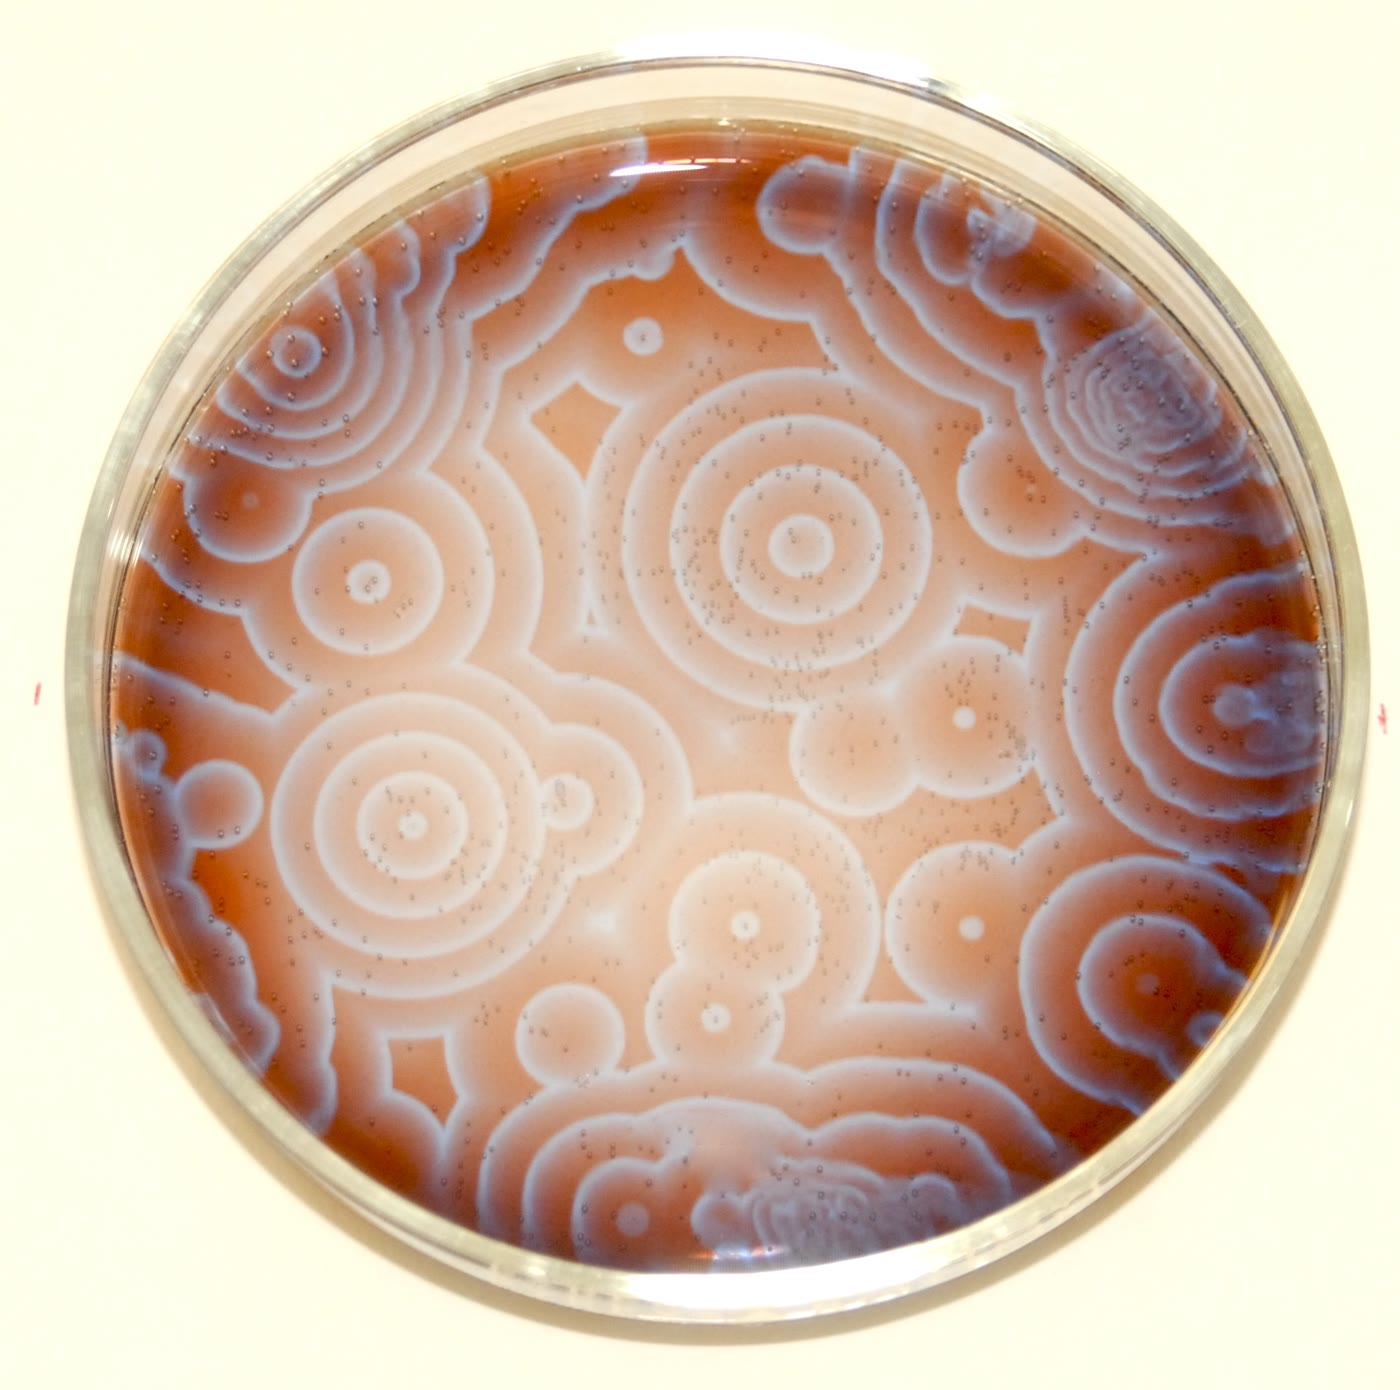
\includegraphics[width=0.48\linewidth]{images/book4/bz-reaction.jpg}

{\small Gelombang spiral reaksi Belousov--Zhabotinsky dalam lapisan tipis
larutan: setiap muka gelombang biru adalah gelombang oksidasi katalis, yang
merambat ke dalam medium tereduksi (merah) dan tidak dapat masuk kembali ke
daerah yang baru saja ditinggalkannya.}
\end{omfigure}

\begin{definition}[Metode relaksasi, waktu relaksasi kimia]\label{def:b3:complex-kinetics:relaxation}
Yang disebut \emph{metode relaksasi}\index{metode relaksasi} adalah metode yang
mengganggu sebuah sistem dalam kesetimbangan secara mendadak (dengan lonjakan
suhu, tekanan, atau medan listrik) lalu mengikuti kembalinya ke kesetimbangan
yang baru. Untuk gangguan yang kecil, simpangannya meluruh secara
eksponensial, dengan \emph{waktu relaksasi kimia}\index{waktu relaksasi kimia}
$\tau$.
\end{definition}

\begin{proposition}[Waktu relaksasi sebuah asosiasi]\label{prop:b3:complex-kinetics:relaxation-time}
Untuk $\mathrm{A + B \rightleftharpoons C}$ ($k_1$, $k_{-1}$), setelah gangguan kecil,
\[
  \frac1\tau = k_1([\mathrm A]_e + [\mathrm B]_e) + k_{-1} .
\]
\end{proposition}

\begin{proof}
Tuliskan $[\mathrm C] = [\mathrm C]_e + x$, $[\mathrm A] = [\mathrm A]_e - x$, $[\mathrm B] = [\mathrm B]_e - x$.
Maka $\dot x =
k_1([\mathrm A]_e - x)([\mathrm B]_e - x) - k_{-1}([\mathrm C]_e + x)$; suku-suku tanpa
$x$ saling meniadakan pada kesetimbangan, dan dengan membuang $x^2$:
$\dot x = -[k_1([\mathrm A]_e + [\mathrm B]_e) + k_{-1}]x$.
\end{proof}

Mengukur $\tau$ pada beberapa konsentrasi memberikan garis $1/\tau$ terhadap
$[\mathrm A]_e +
[\mathrm B]_e$ yang kemiringannya $k_1$ dan perpotongannya $k_{-1}$: kedua tetapan
itu diperoleh dari eksperimen pada sistem yang tidak pernah meninggalkan
kesetimbangan lebih dari beberapa persen. Manfred Eigen mengukur dengan cara
ini reaksi-reaksi tercepat dalam larutan, di antaranya penetralan \ce{H3O+}
oleh \ce{OH-}.

\begin{omfigure}
\begin{tikzpicture}
\begin{axis}[width=0.62\linewidth, height=5.0cm, xmin=0, xmax=780, ymin=0, ymax=1.05,
  axis lines=left, xlabel={$t$ / \unit{\micro s}}, ylabel={$([\mathrm C] - [\mathrm C]_e)/([\mathrm C]_0 - [\mathrm C]_e)$},
  tick label style={font=\small}, label style={font=\small},
  legend style={font=\scriptsize, draw=none, at={(0.97,0.97)}, anchor=north east},
  legend cell align=left]
\addplot[omDef, very thick] table[x=t_us, y=dC] {figdata/out/bachelor-3-chemical-relaxation.dat};
\addplot[omThm, thick, dashed] table[x=t_us, y=exp] {figdata/out/bachelor-3-chemical-relaxation.dat};
\legend{persamaan laju lengkap, {$\eu^{-t/\tau}$, $\tau = \qty{156}{\micro s}$}}
\draw[black!40, densely dotted] (axis cs:156,0) -- (axis cs:156,0.368) -- (axis cs:0,0.368);
\end{axis}
\end{tikzpicture}

{\small Relaksasi $\mathrm{A + B \rightleftharpoons C}$ setelah lonjakan suhu yang
menurunkan tetapan kesetimbangannya sebesar 5\,\% (model:
$k_1 = \qty{1.0e8}{L.mol^{-1}.s^{-1}}$, $k_{-1} = \qty{1.0e3}{s^{-1}}$, seluruhnya
\qty{1.0e-4}{mol/L} A dan B): persamaan laju lengkap dan eksponensial dengan
$1/\tau = k_1([\mathrm A]_e + [\mathrm B]_e) + k_{-1}$ berimpit.}
\end{omfigure}

\begin{definition}[Aliran terhenti, fotolisis kilat]\label{def:b3:complex-kinetics:fast}
Yang disebut \emph{metode aliran terhenti}\index{metode aliran terhenti} adalah
metode yang mencampur dua larutan pereaksi dalam sekitar satu milidetik
dengan mendorongnya melalui sebuah pencampur ke dalam sel pengamatan, lalu
menghentikan alirannya dan merekam absorbans atau \omterm{def:b3:electronic-spectroscopy:luminescence}{fluoresensinya}. Yang
disebut \emph{fotolisis kilat}\index{fotolisis kilat} adalah metode yang
membentuk spesies reaktif dengan pulsa cahaya singkat yang kuat lalu
mengikuti reaksi-reaksinya dengan berkas cahaya kedua yang ditunda.
\end{definition}

\begin{omfigure}
\begin{tikzpicture}[font=\small, >=Stealth]
  % two drive syringes
  \foreach \y/\lab in {1.1/A, -0.1/B}{
    \draw[thick] (0,\y) rectangle (2.2,\y+0.6);
    \fill[omDef!25] (0.6,\y+0.05) rectangle (2.15,\y+0.55);
    \draw[thick] (0.6,\y) -- (0.6,\y+0.6);
    \draw[thick] (-0.6,\y+0.3) -- (0.6,\y+0.3);
    \node at (1.4,\y+0.3) {\lab};
    \draw[thick] (2.2,\y+0.3) -- (2.8,\y+0.3);}
  \draw[thick] (2.8,1.4) -- (3.2,0.8) (2.8,0.2) -- (3.2,0.8);
  \node[draw, thick, circle, minimum size=5mm, fill=white] (mx) at (3.4,0.8) {};
  \node[font=\scriptsize, anchor=north west] at (3.22,0.45) {pencampur};
  \draw[thick] (mx.east) -- (4.4,0.8);
  \draw[thick, fill=omThm!15] (4.4,0.55) rectangle (5.4,1.05);
  \node[font=\scriptsize, anchor=north west, align=left] at (5.0,0.5) {sel\\ pengamatan};
  \draw[->, omThm, thick] (4.9,2.0) -- (4.9,1.1) node[pos=0, above, font=\scriptsize] {cahaya};
  \draw[->, omThm, thick] (4.9,0.5) -- (4.9,-0.4) node[below, font=\scriptsize] {detektor};
  \draw[thick] (5.4,0.8) -- (6.2,0.8);
  \draw[thick] (6.2,0.5) rectangle (7.6,1.1);
  \draw[thick] (7.0,0.5) -- (7.0,1.1);
  \draw[thick] (7.0,0.8) -- (7.9,0.8);
  \draw[thick] (7.9,0.4) -- (7.9,1.2);
  \node[font=\scriptsize, anchor=south] at (6.9,1.15) {semprit penghenti};
  \draw[->, black!60] (-1.2,1.4) -- (-0.7,1.4) node[pos=0, left, font=\scriptsize] {pendorong};
  \draw[->, black!60] (-1.2,0.2) -- (-0.7,0.2);
\end{tikzpicture}

{\small Peralatan aliran terhenti. Pendorong menekan dua semprit; larutan-larutan
bertemu di pencampur dan mengisi sel pengamatan dalam sekitar satu milidetik;
penghisap semprit penghenti membentur sebuah penahan, aliran berhenti, dan
detektor merekam reaksi larutan yang baru dicampur.}
\end{omfigure}

\begin{omfigure}
\begin{tikzpicture}
\begin{axis}[width=0.62\linewidth, height=5.0cm, xmin=0, xmax=20, ymin=0, ymax=5.5,
  axis lines=left, xlabel={$t$ / ms}, ylabel={$[\mathrm P_1]$ / \unit{\micro M}},
  tick label style={font=\small}, label style={font=\small}]
\addplot[omDef, very thick] table[x=t_ms, y=P_uM] {figdata/out/bachelor-3-michaelis-menten-burst.dat};
\addplot[black!45, dashed, domain=0:20] {1.28 + 0.2*x};
\draw[->, black!60] (axis cs:4.5,0.7) -- (axis cs:0.25,1.24);
\node[font=\scriptsize, anchor=west] at (axis cs:4.5,0.7) {amplitudo semburan, \qty{1.28}{\micro M}};
\end{axis}
\end{tikzpicture}

{\small Rekaman semburan aliran terhenti (data soal akhir pekan): produk
pertama \omterm{def:b3:complex-kinetics:enzyme}{enzim} dua tahap muncul dalam semburan cepat yang diikuti garis lurus;
garis putus-putus mengekstrapolasi keadaan tunak kembali ke $t = 0$.}
\end{omfigure}

\begin{inthelab}[Sebuah pengukuran aliran terhenti]
Kedua semprit diisi dengan larutan \omterm{def:b3:complex-kinetics:enzyme}{enzim} dan larutan substrat dalam bufer
yang sama, ditermostatkan, lalu ditembakkan beberapa kali untuk membilas sel
sebelum tembakan-tembakan yang direkam; setiap rekaman dirata-ratakan atas
lima sampai sepuluh tembakan. Waktu mati, yaitu umur campuran ketika
pengamatan dimulai, diukur sekali dengan reaksi yang lajunya diketahui.
\end{inthelab}

\begin{safety}{\ghs[0.8cm]{GHS05}\ghs[0.8cm]{GHS06}\ghs[0.8cm]{GHS09}}
% ledger: ghs4:Br2
Bromin: cairan merah kecokelatan yang mudah menguap dan berat; fatal jika
terhirup, menyebabkan luka bakar parah, sangat beracun bagi kehidupan
akuatik. Hanya ditangani di lemari asam, dengan sarung tangan dan pelindung
wajah; larutan natrium tiosulfat disiapkan di dekatnya untuk mereduksi
tumpahan.
\end{safety}

\begin{history}[Bodenstein dan Belousov]
Max Bodenstein dan Samuel Lind mengukur hukum laju hidrogen--bromin pada tahun
1906; Jens Christiansen, Karl Herzfeld, dan Michael Polanyi menjelaskannya pada
tahun 1919 dengan mekanisme berantai dalam bab ini. Boris Belousov, seorang
biokimiawan di Moskwa, menemukan \omterm{def:b3:complex-kinetics:oscillating}{reaksi berosilasinya} sekitar tahun 1951
ketika mencari model kimia untuk sebuah siklus metabolik; naskahnya ditolak,
dan hanya sebuah abstrak singkat yang terbit pada tahun 1959. Anatol
Zhabotinsky melanjutkan kajian reaksi itu pada tahun 1960-an dan
menjelaskannya; mekanisme lengkapnya disusun pada awal tahun 1970-an.
\end{history}

\section{Latihan}

\begin{exercise}[$\star$]\label{exo:b3:complex-kinetics:1}
Untuk rantai $\ce{Cl2 -> 2 Cl}$, $\ce{Cl + H2 -> HCl + H}$, $\ce{H + Cl2 -> HCl + Cl}$,
$\ce{2 Cl -> Cl2}$, namailah setiap tahap dan pembawa-pembawa rantainya, lalu
tuliskan reaksi keseluruhannya.
\end{exercise}

\begin{exercise}[$\star$]\label{exo:b3:complex-kinetics:2}
Sebuah sistem Lindemann mempunyai $k_2 = \qty{1.0e7}{s^{-1}}$ dan
$k_{-1} = \qty{1.0e10}{L.mol^{-1}.s^{-1}}$ (data latihan). Hitunglah $[\mathrm M]_{1/2}$
dan tekanan yang bersesuaian pada \qty{750}{K}.
\end{exercise}

\begin{exercise}[$\star$]\label{exo:b3:complex-kinetics:3}
Nyatakan $v/V_{\max}$ pada $[\mathrm S] = K_M$, $3K_M$ dan $9K_M$. Konsentrasi
berapa yang memberikan 90\,\% dari $V_{\max}$?
\end{exercise}

\begin{exercise}[$\star$]\label{exo:b3:complex-kinetics:4}
% ledger: enz:median.kcatKM, visc:H2O.25C
Sebuah \omterm{def:b3:complex-kinetics:enzyme}{enzim} mempunyai $k_{\mathrm{cat}} = \qty{100}{s^{-1}}$ dan $K_M = \qty{0.80}{mM}$.
Hitunglah \omterm{def:b3:complex-kinetics:michaelis}{tetapan spesifisitasnya} dan bandingkan dengan batas difusi dalam
air, \qty{7.4e9}{L.mol^{-1}.s^{-1}}, serta dengan nilai khas
$10^5$~\unit{L.mol^{-1}.s^{-1}}.
\end{exercise}

\begin{exercise}[$\star\star$]\label{exo:b3:complex-kinetics:5}
Dekomposisi $\ce{CH3CHO -> CH4 + CO}$ diusulkan berlangsung melalui: $\ce{CH3CHO -> CH3 +
CHO}$ ($k_1$); $\ce{CH3 + CH3CHO -> CH4 + CH3CO}$ ($k_2$); $\ce{CH3CO -> CH3 + CO}$ ($k_3$);
$\ce{2 CH3 -> C2H6}$ ($k_4$). Tunjukkan bahwa laju pembentukan metana adalah
$k_2(k_1/2k_4)^{1/2}[\ce{CH3CHO}]^{3/2}$.
\end{exercise}

\begin{exercise}[$\star\star$]\label{exo:b3:complex-kinetics:6}
Dimulai dari konsentrasi \ce{H2} dan \ce{Br2} yang sama, dengan $k' = 0.10$,
dengan faktor berapa lajunya telah turun ketika setengah bromin terpakai?
Berapa bagian dari penurunan itu yang disebabkan oleh inhibisi?
\end{exercise}

\begin{exercise}[$\star\star$]\label{exo:b3:complex-kinetics:7}
Dalam sebuah model campuran hidrogen--oksigen (data latihan), percabangan
mempunyai tetapan laju $f = 1000\,p$, terminasi di dinding $6000/p$, dan
terminasi tiga benda $10\,p^2$, semuanya dalam \unit{s^{-1}} dengan $p$ dalam kPa.
Carilah rentang tekanan tempat campuran itu meledak.
\end{exercise}

\begin{exercise}[$\star\star$]\label{exo:b3:complex-kinetics:8}
Laju awal adalah $\qty{0.20}{\micro M.s^{-1}}$ pada $[\mathrm S] = \qty{0.50}{mM}$ dan
$\qty{0.40}{\micro M.s^{-1}}$ pada \qty{2.0}{mM}. Carilah $K_M$ dan $V_{\max}$.
\end{exercise}

\begin{exercise}[$\star\star$]\label{exo:b3:complex-kinetics:9}
Dengan \qty{50}{\micro M} sebuah inhibitor, garis Lineweaver--Burk sebuah \omterm{def:b3:complex-kinetics:enzyme}{enzim}
($K_M = \qty{0.80}{mM}$) bertemu dengan garis tanpa inhibisi pada sumbu $1/v$
dan memotong sumbu $1/[\mathrm S]$ pada \qty{-0.417}{mM^{-1}}. Kenalilah jenis
inhibisinya dan hitunglah $K_i$.
\end{exercise}

\begin{exercise}[$\star\star\star$]\label{exo:b3:complex-kinetics:10}
Untuk $\mathrm{A + X \to 2\,X}$ dengan $k = \qty{0.50}{L.mol^{-1}.s^{-1}}$, $a_0 = \qty{1.00}{mol/L}$
dan $x_0 = \qty{0.010}{mol/L}$, hitunglah waktu ketika setengah jumlah akhir X
telah terbentuk, dan waktu \omterm{def:b3:complex-kinetics:michaelis}{laju maksimum}.
\end{exercise}

\begin{exercise}[$\star\star\star$]\label{exo:b3:complex-kinetics:11}
Untuk Brusselator dengan $A = 1$, hitunglah \omterm{def:b3:quantum-model-systems:operator}{nilai-nilai eigen} matriks Jacobi pada
keadaan tunak untuk $B = 1.5$ dan $B = 2.5$, lalu gambarkan perilaku di dekat
keadaan tunak pada masing-masing kasus.
\end{exercise}

\begin{exercise}[$\star\star\star$]\label{exo:b3:complex-kinetics:12}
Untuk $\mathrm{A + B \rightleftharpoons C}$ dengan $k_1 = \qty{1.0e8}{L.mol^{-1}.s^{-1}}$ dan
$k_{-1} = \qty{1.0e3}{s^{-1}}$, serta $[\mathrm A]_e = [\mathrm B]_e = \qty{2.70e-5}{mol/L}$,
hitunglah $\tau$. Bagaimana kedua tetapan laju itu dapat diperoleh hanya dari
pengukuran relaksasi?
\end{exercise}

\section{Soal: Sebuah Enzim, Sebuah Inhibitor, dan Sebuah Dosis}

\begin{problem}[{Soal akhir pekan --- sebuah enzim, sebuah inhibitor, dan sebuah
dosis: parameter Michaelis--Menten dengan kuadrat terkecil, tetapan inhibisi
sebuah inhibitor kompetitif, aktivitas yang tersisa pada dosis tertentu, dan
semburan aliran terhenti}]
\label{pb:b3:complex-kinetics:1}
% ledger: enz:median.kcatKM
Sebuah \omterm{def:b3:complex-kinetics:enzyme}{enzim} ($[\mathrm E]_0 = \qty{5.0}{nM}$ dalam pengujian) menghidrolisis
substratnya; laju-laju awalnya (data soal):
\begin{center}\small
\begin{tabular}{lccccccc}
\hline
$[\mathrm S]$ / mM & 0.10 & 0.20 & 0.40 & 0.80 & 1.60 & 3.20 & 6.40 \\
$v$ / \unit{\micro M.s^{-1}} & 0.0566 & 0.0981 & 0.169 & 0.247 & 0.340 & 0.397 & 0.447 \\ \hline
\end{tabular}
\end{center}
Dengan adanya sebuah inhibitor, pencocokan yang sejenis memberikan $V_{\max}$ yang
tidak berubah dan $K_M$ semu: 0.79, 1.47, 2.38 dan \qty{4.02}{mM} pada
$[\mathrm I] = 0$, 20, 50 dan
\qty{100}{\micro M}. Eksperimen aliran terhenti dengan $[\mathrm E]_0 = \qty{2.0}{\micro M}$
dan substrat jenuh memberikan rekaman semburan pada gambar subbab 5 (semburan
sebesar \qty{1.28}{\micro M} dengan tetapan laju \qty{625}{s^{-1}}, lalu
\qty{200}{\micro M.s^{-1}}).

\medskip\noindent\textbf{Bagian I --- $K_M$ dan $V_{\max}$.}
\begin{enumerate}[beginpenalty=10000]
  \item Mengapa laju awal yang dipakai?
  \item Gambarlah grafik Lineweaver--Burk; garis kuadrat terkecilnya memberikan
        $K_M =
        \qty{0.773}{mM}$ dan $V_{\max} = \qty{0.491}{\micro M.s^{-1}}$. Titik-titik mana
        yang mendominasinya?
  \item Mengapa pencocokan taklinear langsung lebih disukai?
  \item Pencocokan taklinear memberikan $K_M = 0.801 \pm \qty{0.023}{mM}$ dan
        $V_{\max} = 0.502 \pm
        \qty{0.005}{\micro M.s^{-1}}$. Apakah nilai-nilai Lineweaver--Burk sesuai
        dengannya?
  \item Hitunglah $k_{\mathrm{cat}}$.
  \item Hitunglah \omterm{def:b3:complex-kinetics:michaelis}{tetapan spesifisitasnya}.
  \item Bandingkan dengan batas difusi dan dengan \omterm{def:b3:complex-kinetics:enzyme}{enzim} yang khas.
\end{enumerate}

\medskip\noindent\textbf{Bagian II --- Inhibitornya.}
\begin{enumerate}[resume, beginpenalty=10000]
  \item Jenis inhibisi apa yang diperlihatkan data itu?
  \item Tuliskan $K_M^{\mathrm{app}}$ sebagai fungsi $[\mathrm I]$.
  \item Garis kuadrat terkecil $K_M^{\mathrm{app}}$ terhadap $[\mathrm I]$ mempunyai
        perpotongan \qty{0.799}{mM} dan kemiringan \qty{0.0321}{mM.\micro M^{-1}}.
        Simpulkan $K_i$.
  \item Galat bakunya \qty{0.9}{\micro M}. Berikan selang 95\,\% ($t = 4.30$ untuk
        dua derajat kebebasan).
  \item Apa yang diukur oleh $K_i$?
\end{enumerate}

\medskip\noindent\textbf{Bagian III --- Aktivitas yang tersisa.}
\begin{enumerate}[resume, beginpenalty=10000]
  \item Nyatakan fraksi aktivitas yang tersisa, $v_i/v_0$, sebagai fungsi
        $[\mathrm S]$ dan $[\mathrm I]$.
  \item Hitunglah nilainya pada $[\mathrm S] = K_M$ dan $[\mathrm I] = K_i$.
  \item Pada $[\mathrm S] = K_M$ dan $[\mathrm I] = 10K_i$.
  \item Pada $[\mathrm S] = 10K_M$ dan $[\mathrm I] = 10K_i$. Berikan komentar.
  \item Tunjukkan bahwa inhibisi 90\,\% pada $[\mathrm S] = K_M$ memerlukan
        $[\mathrm I] = 18K_i$.
  \item Hitunglah konsentrasi itu dengan $K_i$ hasil pencocokan.
\end{enumerate}

\medskip\noindent\textbf{Bagian IV --- Semburan.}
\begin{enumerate}[resume, beginpenalty=10000]
  \item \omterm{def:b3:complex-kinetics:enzyme}{Enzim} itu bekerja dalam dua tahap, $\mathrm{E + S \to E{-}acyl + P_1}$ ($k_2$)
        lalu $\mathrm{E{-}acyl \to E +
        P_2}$ ($k_3$). Mengapa $\mathrm P_1$ muncul dalam semburan?
  \item Amplitudo semburan adalah $[\mathrm E]_0\bigl(k_2/(k_2 + k_3)\bigr)^2$.
        Simpulkan $k_2/(k_2 + k_3)$.
  \item Dari kemiringan yang tunak, hitunglah $k_{\mathrm{cat}}$ dan bandingkan dengan
        Bagian I.
  \item Tetapan laju semburan adalah $k_2 + k_3$. Simpulkan $k_2$ dan $k_3$.
  \item Periksalah bahwa $k_{\mathrm{cat}} = k_2k_3/(k_2 + k_3)$.
  \item Nyatakan hasilnya: konsentrasi inhibitor yang memberikan inhibisi
        90\,\% pada $[\mathrm S] = K_M$.
\end{enumerate}
\end{problem}
